%%%%%%%%%%%%%%%%%%%%%%%%%%%%%%%%%%%%%%%%%%%%%%%%%%%%%%%%%%%%%%%%%%%%%%%%%%%%%%%%%%%
%% This project aims to create the UFC template for presentation.                %%
%% author: Maurício Moreira Neto - Doctoral student in Computer Science (MDCC)   %%
%% contacts:                                                                     %%
%%    e-mail: maumneto@ufc.br                                                    %%
%%    linktree: https://linktr.ee/maumneto                                       %%
%%%%%%%%%%%%%%%%%%%%%%%%%%%%%%%%%%%%%%%%%%%%%%%%%%%%%%%%%%%%%%%%%%%%%%%%%%%%%%%%%%%
\documentclass{libs/ufc_format}
% Inserting the preamble file with the packages
%%%%%%%%%%%%%%%%%%%%%%%%%%%%%%%%%%%%%%%%%%%%%%%%%%%%%%%%%%%%%%%%%%%%%
%% This file contains the packages that can be used in the beamer. %%
%%%%%%%%%%%%%%%%%%%%%%%%%%%%%%%%%%%%%%%%%%%%%%%%%%%%%%%%%%%%%%%%%%%%%
% Package to fonts family
\usepackage[T1]{fontenc}
% Package to accentuation
\usepackage[utf8]{inputenc}
% Package to Portuguese language
\usepackage[brazil]{babel}
% Package to Figures
\usepackage{graphicx}
% Package to the colors
\usepackage{color}
% Package to the colors
\usepackage{xcolor}
% Packages to math symbols and expressions
\usepackage{amsfonts, amssymb, amsmath}
% Package to multiple lines and columns in table
\usepackage{multirow, array} 
% Package to create pseudo-code
% For more detail of this package: http://linorg.usp.br/CTAN/macros/latex/contrib/algorithm2e/doc/algorithm2e.pdf
\usepackage{algorithm2e}
% Package to insert code
\usepackage{listings} 
\usepackage{keyval}
% Package to justify text
\usepackage[document]{ragged2e}
% Package to manage the bibliography
\usepackage[backend=biber, style=numeric, sorting=none]{biblatex}
% Package to facilities quotations
\usepackage{csquotes}
% Package to use multicols
\usepackage{multicol}

\usepackage{hyperref}

\renewcommand*\footnoterule{}
\renewcommand{\footnotelayout}{\raggedleft}

% Inserting the references file
\bibliography{references.bib}

% Title
\title[Trabalho de Conclusão de Curso]{\textbf{Um estudo comparativo entre tecnologias de \textit{back-end}: Node.js, Django REST Framework e ASP.NET Core}}
% Subtitle
%\subtitle{Trabalho de Conclusão de Curso}
% Author of the presentation
\author{Klayver Ximenes Carmo}

% Institute's Name
\institute[UFC]{
    % email for contact
    % \normalsize{\email{klayver@alu.ufc.br}}
    \orientador{Prof. Dr. Fischer Jônatas Ferreira}
    \newline
    % Department Name
    \department{Curso de graduação em Engenharia de Computação}
    \newline
    % university name
    \ufc
}
% date of the presentation
\date{28 de novembro de 2023}


%%%%%%%%%%%%%%%%%%%%%%%%%%%%%%%%%%%%%%%%%%%%%%%%%%%%%%%%%%%%%%%%%%%%%%%%%%%%%%%%%%
%% Start Document of the Presentation                                           %%               
%%%%%%%%%%%%%%%%%%%%%%%%%%%%%%%%%%%%%%%%%%%%%%%%%%%%%%%%%%%%%%%%%%%%%%%%%%%%%%%%%%
\begin{document}
% insert the code style
%%%%%%%%%%%%%%%%%%%%%%%%%%%%%%%%%%%%%%%%%%%%%%%%%%%%%%%%%%%%%%%%%%%%%%%%%%%%%%%%%%%
%% This file contains the style of the codes show in slides.                     %%
%% The package used is listings, but it possible to used others.                 %%
%%%%%%%%%%%%%%%%%%%%%%%%%%%%%%%%%%%%%%%%%%%%%%%%%%%%%%%%%%%%%%%%%%%%%%%%%%%%%%%%%%%

% color used in the code style
\definecolor{codegreen}{rgb}{0,0.6,0}
\definecolor{codegray}{rgb}{0.5,0.5,0.5}
\definecolor{codepurple}{rgb}{0.58,0,0.82}
\definecolor{codebackground}{rgb}{0.95,0.95,0.92}

% style of the code!
\lstdefinestyle{codestyle}{
    backgroundcolor=\color{codebackground},   
    commentstyle=\color{codegreen},
    keywordstyle=\color{magenta},
    numberstyle=\tiny\color{codegray},
    stringstyle=\color{codepurple},
    basicstyle=\ttfamily\footnotesize,
    frame=single,
    breakatwhitespace=false,         
    breaklines=true,                 
    captionpos=b,                    
    keepspaces=true,                 
    numbers=left,                    
    numbersep=5pt,                  
    showspaces=false,                
    showstringspaces=false,
    showtabs=false,                  
    tabsize=2,
    title=\lstname 
}

\lstset{style=codestyle}


%% ---------------------------------------------------------------------------
% First frame (with tile, subtitle, ...)
\begin{frame}{}
    \maketitle
\end{frame}

%% ---------------------------------------------------------------------------
% Second frame
\begin{frame}{Sumário}
    % \begin{multicols}{2}
        \tableofcontents
    % \end{multicols}
\end{frame}

%% ---------------------------------------------------------------------------
% This presentation is separated by sections and subsections
\section{Introdução}

\begin{frame}{Contexto}
    \begin{itemize}
        \item O desenvolvimento Web teve início na década de 90 com a criação dos primeiros sites;
        \vspace*{0.5em}
        \item Com o passar do tempo o desenvolvimento Web ficou mais dinâmico e interativo;
        \vspace*{0.5em}
        \item Surgimento dos termos \textit{front-end} e \textit{back-end};
        \vspace*{0.5em}
        \item Com esta camada é possível gerenciar servidores, bancos de dados, processar e armazenar dados.
    \end{itemize}
\end{frame}

\begin{frame}{Contexto}
    \begin{figure}[H]
        \centering
        \caption{Frameworks \textit{back-end}}
        
\includegraphics[width=0.9\linewidth]{figuras/tech-backend.pdf}
        \captionsetup{justification=centering}
        \source{O autor.}
        \label{fig:tech-backend}    
    \end{figure}
\end{frame}

\begin{frame}{Contexto}
    Em 2022, o StackOverflow conduziu uma pesquisa com mais de 70 mil desenvolvedores, elencando os \textit{frameworks} mais utilizados\nocite{StackOverflowSurvey}\let\thefootnote\relax\footnotetext{\href{https://survey.stackoverflow.co/2022/\#technology-most-popular-technologies}{Stack Overflow Annual Developer Survey}}.
    \begin{figure}[H]
        \centering
        \caption{Frameworks \textit{back-end}}
        
\includegraphics[width=0.9\linewidth]{figuras/tech-backend-selecionadas.pdf}
        \captionsetup{justification=centering}
        \source{O autor.}
        \label{fig:tech-backend2}    
    \end{figure}
\end{frame}

\begin{frame}{Objetivo}
    A definição dos objetivos foram feitos com base no modelo objetivo-questão-métrica (GQM)\nocite{6156}\let\thefootnote\relax\footnotetext{\scriptsize\href{https://ieeexplore.ieee.org/document/6156}{GQM - The TAME project: towards improvement-oriented software environments}}.

    Foram \textbf{comparados} \textit{frameworks} \textit{back-end} de maneira teórica e prática; 

    \textbf{com a finalidade} de i) identificar funcionalidades nativas em fase de desenvolvimento e ii) analisar sua performance e desempenho;

    \textbf{no que diz respeito} a auxiliar profissionais e pesquisadores na escolha da abordagem mais adequada para suas estratégias;

    \textbf{sob a perspectiva} de desenvolvedores e pesquisadores na área de desenvolvimento \textit{back-end} no contexto de construção e estudo de aplicações Web.
\end{frame}

% \begin{frame}{Objetivos}
%     Objetivo Geral:
%     \begin{itemize}
%         \item Analisar e comparar os \textit{frameworks} de \textit{back-end}: Node.js, Django REST Framework e ASP.NET Core. 
%             Pontuando características/funcionalidades que são presenciadas em tempo de desenvolvimento e comparar resultados práticos em diferentes cenários.
%             Assim como, relatar o aprendizado e resultados obtidos no desenvolvimento de um \textit{software} alvo destinado ao controle de estoque do laboratório.
%     \end{itemize}
% \end{frame}

\begin{frame}{Objetivos Específicos}
     \begin{itemize}
        \item Realizar estudos teóricos sobre os \textit{frameworks};
        \vspace*{0.5em}
        \item Pontuar características de desenvolvimento entre os \textit{frameworks};
        \vspace*{0.5em}
        \item Desenvolver um \textit{software} alvo utilizando os \textit{frameworks} em estudo;
        \vspace*{0.5em}
        \item Aplicar e analisar métricas com base no \textit{software} alvo desenvolvido.
    \end{itemize}
\end{frame}

\begin{frame}{Motivação}
    Com base em pesquisas bibliográficas, até o momento, não foram encontrados estudos comparativos focados à avaliação das compatibilidades/funcionalidades teóricas e à análise de cenários práticos de testes nos três \textit{frameworks} em estudo.
\end{frame}

%% ---------------------------------------------------------------------------
\section{Fundamentação Teórica}
\begin{frame}{Fundamentação Teórica}
    \begin{figure}[H]
        \centering
        \caption{Modelo arquitetural de uma API REST}
        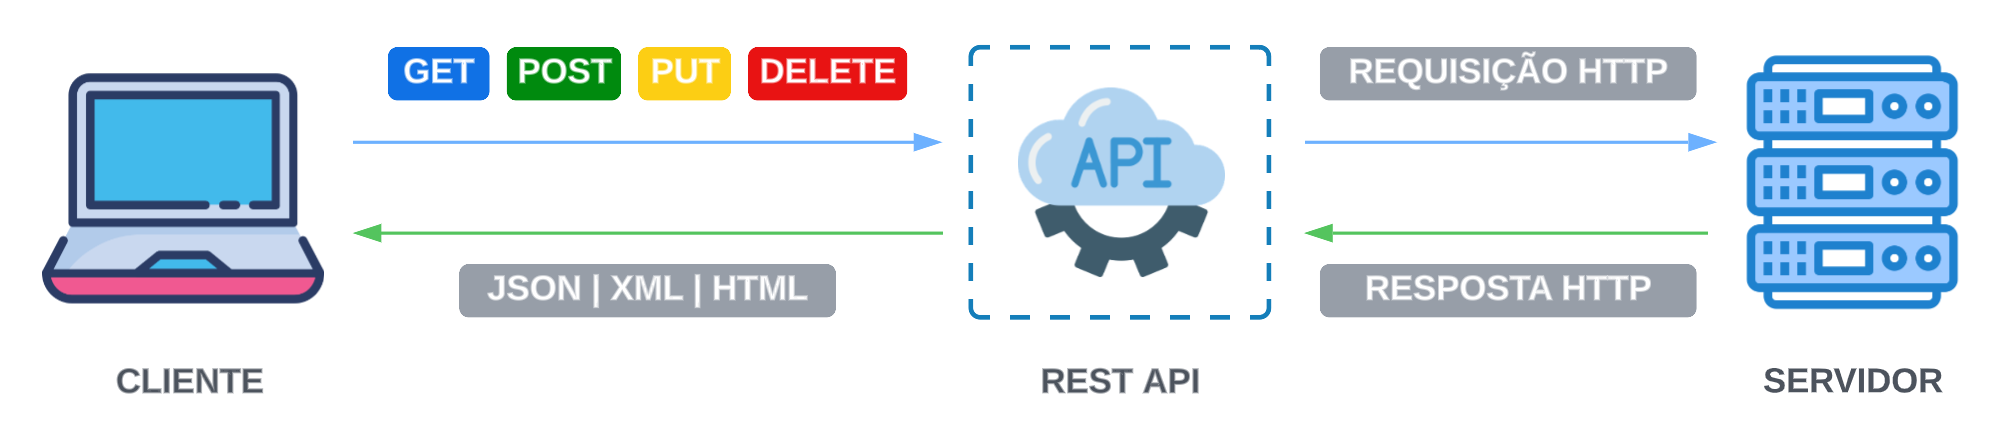
\includegraphics[width=1\linewidth]{figuras/modelo-rest-api.png}
        \captionsetup{justification=centering}
        \source{O autor.}
        \label{fig:modelo-rest-api}
    \end{figure}
\end{frame}

\begin{frame}{Fundamentação Teórica}
    \textbf{Node.js}\nocite{nodejs}\let\thefootnote\relax\footnotetext{\url{https://nodejs.org/}}
    \begin{multicols}{2}
        \begin{itemize}
            \item O Node.js é um \textit{framework} baseado em JavaScript;
            \item Foi construído sobre a \textit{engine} V8 para o Chrome;
            \item Modelo de programação: Assíncrono e orientado a eventos.
        \end{itemize}
        \begin{figure}[H]
            \centering
            % \caption{Modelo arquitetural de uma API REST}
            
\includegraphics[width=0.8\linewidth]{figuras/logo-nodejs.pdf}
            \captionsetup{justification=centering}
            % \source{O autor.}
            \label{fig:modelo-rest-api}
        \end{figure}
    \end{multicols}
\end{frame}

\begin{frame}{Fundamentação Teórica}
    \textbf{Django REST Framework}\nocite{django}\let\thefootnote\relax\footnotetext{\url{https://www.djangoproject.com}}
    \begin{multicols}{2}
    \begin{itemize}
        \item É um \textit{framework} Web baseado na linguagem Python;
        \item DRF funciona sob a estrutura do Django;
        \item Versão do Django voltada para o desenvolvimento de APIs;
    \end{itemize}
        \begin{figure}[H]
            \centering
            % \caption{Modelo arquitetural de uma API REST}
            
\includegraphics[width=1\linewidth]{figuras/logo-drf.pdf}
            \captionsetup{justification=centering}
            % \source{O autor.}
            \label{fig:modelo-rest-api}
        \end{figure}
    \end{multicols}
\end{frame}

\begin{frame}{Fundamentação Teórica}
    \textbf{ASP.NET Core}\nocite{dotnet}\let\thefootnote\relax\footnotetext{\url{https://learn.microsoft.com/en-us/aspnet/core}}
    \begin{multicols}{2}
        \begin{itemize}
            \item Linguagem principal: C\#;
            \item Framework multiplataforma desenvolvido pela Microsoft;
            \item Modelo de programação: Orientado a Objetos;
        \end{itemize}
        \begin{figure}[H]
            \centering
            % \caption{Modelo arquitetural de uma API REST}
            
\includegraphics[width=0.7\linewidth]{figuras/logo-dotnet.pdf}
            \captionsetup{justification=centering}
            % \source{O autor.}
            \label{fig:modelo-rest-api}
        \end{figure}
    \end{multicols}
\end{frame}

\begin{frame}{Testes de carga}
    \textbf{Cenários de teste}\nocite{7123673}\let\thefootnote\relax\footnotetext{\href{https://ieeexplore.ieee.org/document/7123673}{A Survey on Load Testing of Large-Scale Software Systems}}
    \begin{itemize}
        \item Teste de pico
            \begin{itemize}
                \item Um servidor é submetido à uma grande quantidade de requisições durante um curto intervalo de tempo;
            \end{itemize}
        \vspace*{0.5em}
        \item Teste de carga crescente
            \begin{itemize}
                \item Um servidor é submetido à uma carga crescente de requisições e monitorada para analisar o comportamento sob esta situação.
            \end{itemize}
        \vspace*{0.5em}
        \item Teste de resistência
            \begin{itemize}
                \item Um servidor é submetido a uma carga constante durante um longo período de tempo, buscando identificar o comportamento geral do sistema.
            \end{itemize}
    \end{itemize}
\end{frame}

%% ---------------------------------------------------------------------------
\section{Metodologia}
\begin{frame}{Questões de pesquisa}
    \textit{\textbf{QP\textsubscript{1}:} Qual é o \textit{framework} com mais funcionalidades nativas seguindo as características escolhidas para estudo?}\\
    \vspace*{0.5em}
    \textbf{Cenário 1 - Teste de pico}
    \begin{itemize}
        \item \textit{\textbf{QP\textsubscript{2}:} Qual é o \textit{framework} mais otimizado com relação ao \underline{consumo de recursos} no cenário de teste de pico?}
        \vspace*{0.5em}
        \item \textit{\textbf{QP\textsubscript{3}:} Qual é o \textit{framework} mais otimizado com relação ao \underline{tempo de resposta} no cenário de teste de pico?}
    \end{itemize}
\end{frame}

\begin{frame}{Questões de pesquisa}
    \textbf{Cenário 2 - Teste de carga crescente}
    \begin{itemize}
        \item \textit{\textbf{QP\textsubscript{4}:} Qual é o \textit{framework} mais otimizado com relação ao \underline{consumo de recursos} no cenário de teste de carga crescente?}
        \item \textit{\textbf{QP\textsubscript{5}:} Qual é o \textit{framework} mais otimizado com relação ao \underline{tempo de resposta} no cenário de teste de carga crescente?}
    \end{itemize}
    \vspace*{0.5em}
    \textbf{Cenário 3 - Teste de resistência}
    \begin{itemize}
        \item \textit{\textbf{QP\textsubscript{6}:} Qual é o \textit{framework} mais otimizado com relação ao \underline{consumo de recursos} no cenário de teste de resistência?}
        \item \textit{\textbf{QP\textsubscript{7}:} Qual é o \textit{framework} mais otimizado com relação ao \underline{tempo de resposta} no cenário de teste de resistência?}
    \end{itemize}
\end{frame}

\begin{frame}{Metodologia}
    \begin{figure}[H]
        \centering
        \caption{Etapas metodológicas}
        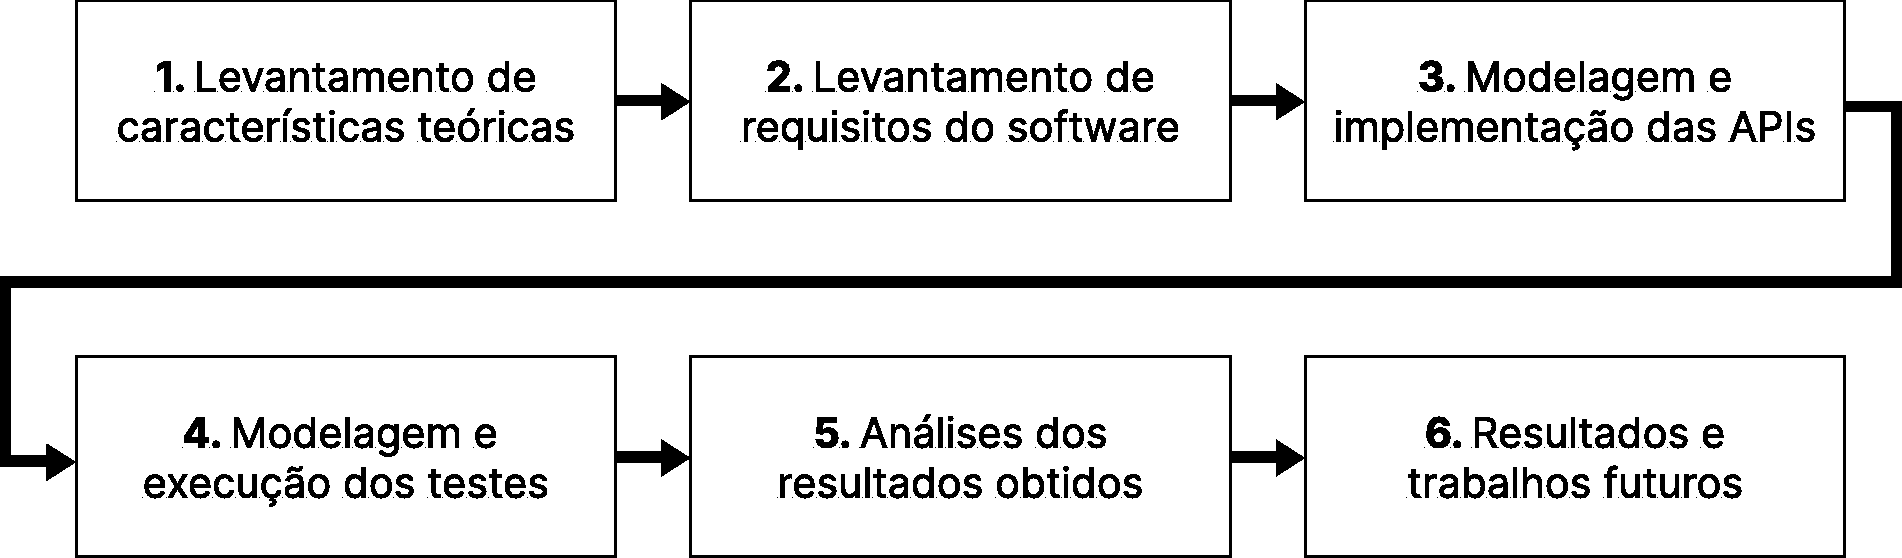
\includegraphics[width=1\linewidth]{figuras/diagrama-atividades2linhas.pdf}
        \captionsetup{justification=centering}
        \source{O autor.}
        \label{fig:etapas-metodologicas}
    \end{figure}
\end{frame}


\begin{frame}{Metodologia}
    \textbf{A partir de uma revisão bibliográfica foram definidas as seguintes características teóricas para comparação:}
    \begin{itemize}
        \item Suporte a diferentes sistemas operacionas;
            \begin{itemize}
                \item Windows;
                \item Linux;
                \item MacOS;
            \end{itemize}
        \item Suporte a bancos de dados;
            \begin{itemize}
                \item MySQL;
                \item PostgreSQL;
                \item SQLite;
                \item MongoDB;
                \item SQL Server;
            \end{itemize}
        \item Suporte a ORM nativo;
        \item Documentação nativa da API em tempo de desenvolvimento.
    \end{itemize} 
\end{frame}

\begin{frame}{Metodologia}
    \textbf{Levantamento de requisitos do \textit{software} alvo}
    \begin{figure}[H]
        \centering
        \caption{Diagrama do \textit{software} alvo}
        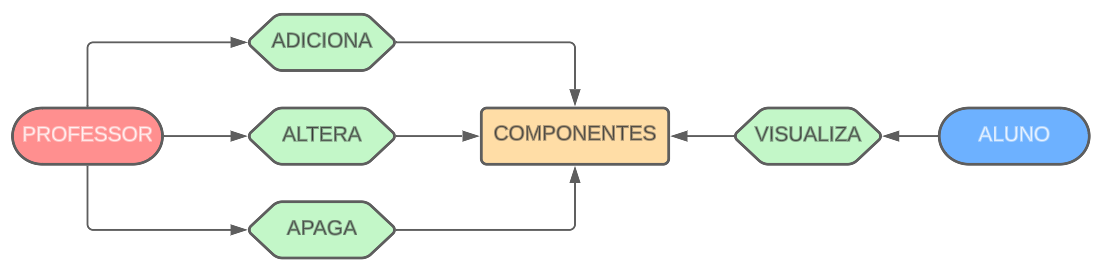
\includegraphics[width=1\linewidth]{figuras/diagama-soft-alvo.png}
        \captionsetup{justification=centering}
        \source{O autor.}
        \label{fig:diagrama-soft-alvo}
    \end{figure}
\end{frame}

\begin{frame}{Metodologia - modelagem do \textit{software} alvo}
    \begin{table}[h!] 
        \centering
        \captionsetup{justification=centering}
        \caption{Métodos do \textit{software} alvo}
        \begin{tabular}{ccc}
            \hline
            \textbf{Método} & \textbf{Ação} & \textbf{Exemplo de uso} \\ \hline
            GET & Ler & Buscar informações dos componentes \\ 
            POST & Criar & Inserir um componente na base de dados \\ 
            PUT & Atualizar & Alterar informações de um componente \\ 
            DELETE & Apagar & Remover um componente da base de dados \\ 
            \hline
        \end{tabular}
        \label{tab:metodos-http}
    \end{table}
\end{frame}

\begin{frame}{Metodologia}
    \textbf{Métricas comparativas práticas}
    \begin{itemize}
        \item Taxa de erros de requisição
            \begin{itemize}
                \item Essencial para analisar a proporção de solicitações que resultam em erros em relação ao número total de solicitações feitas durante os testes;
            \end{itemize}
        \item Tempo de requisição
            \begin{itemize}
                \item Importante para medir o tempo que uma API leva para responder ou completar uma solicitação de um cliente;
            \end{itemize}
        \item Consumo de memória RAM
            \begin{itemize}
                \item Verificar o quanto de memória é consumido durante a execução das solicitações.
            \end{itemize}
        \item Consumo de CPU
            \begin{itemize}
                \item Similar ao consumo de memória, verifica o gerenciamento de recursos de uma aplicação com relação a CPU;
            \end{itemize}
    \end{itemize}
\end{frame}

% \begin{frame}{Modelagem dos testes}
%     \textbf{Fluxo de requisições dos testes}
%     \begin{enumerate}
%         \item Criar um componente no banco de dados;
%         \item Atualizar os dados do componente criado no passo anterior;
%         \item Fazer a leitura do componente criado;
%         \item Apagar o componente criado no passo 1;
%     \end{enumerate}
% \end{frame}

\begin{frame}{Modelagem dos testes}
    \begin{figure}[H]
        \centering
        \caption{Fluxo de requisições dos testes}
        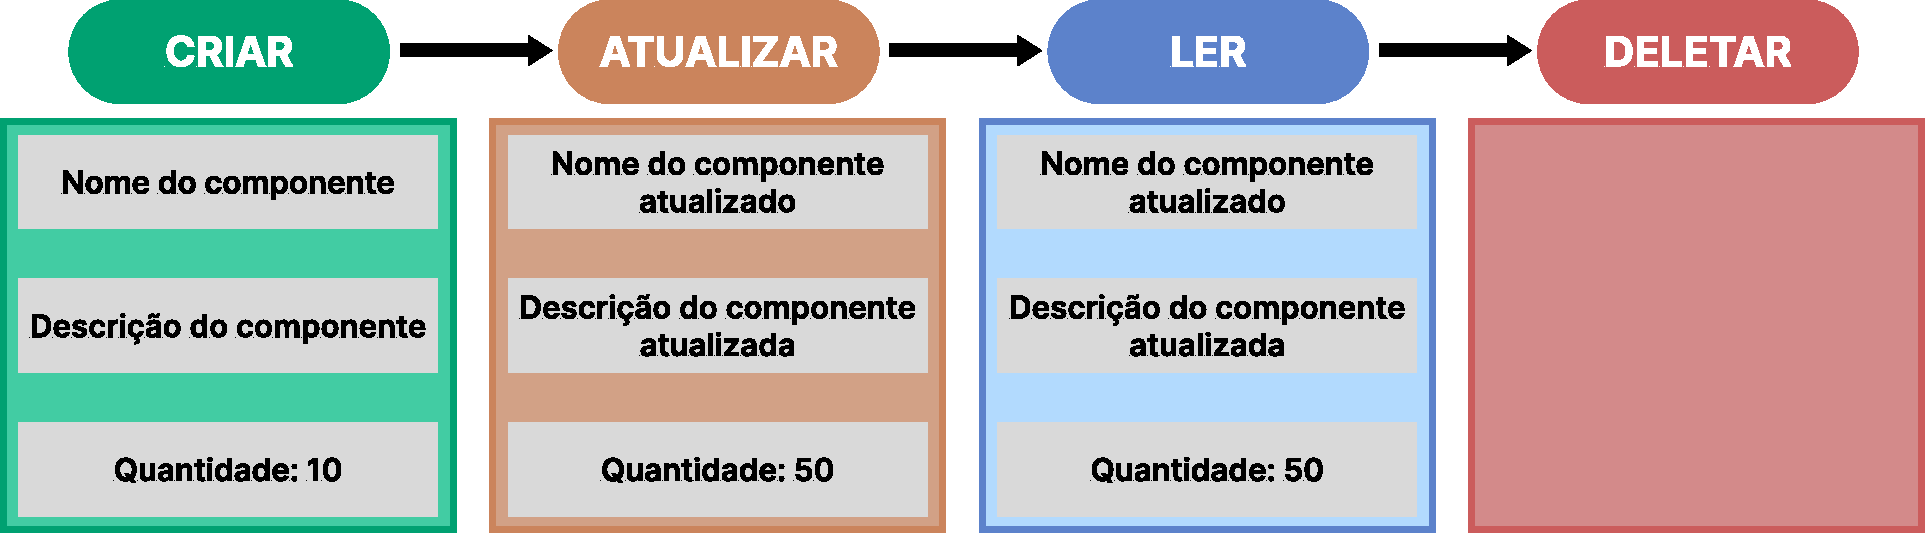
\includegraphics[width=1\linewidth]{figuras/fluxo-requisicoes-testes.pdf}
        \captionsetup{justification=centering}
        \source{O autor.}
        \label{fig:fluxo-requisicoes-testes}
    \end{figure}
\end{frame}

% \begin{frame}{Modelagem dos cenários de teste}
%     \begin{figure}[H]
%         \centering
%         \caption{Modelagem do teste de pico}
%         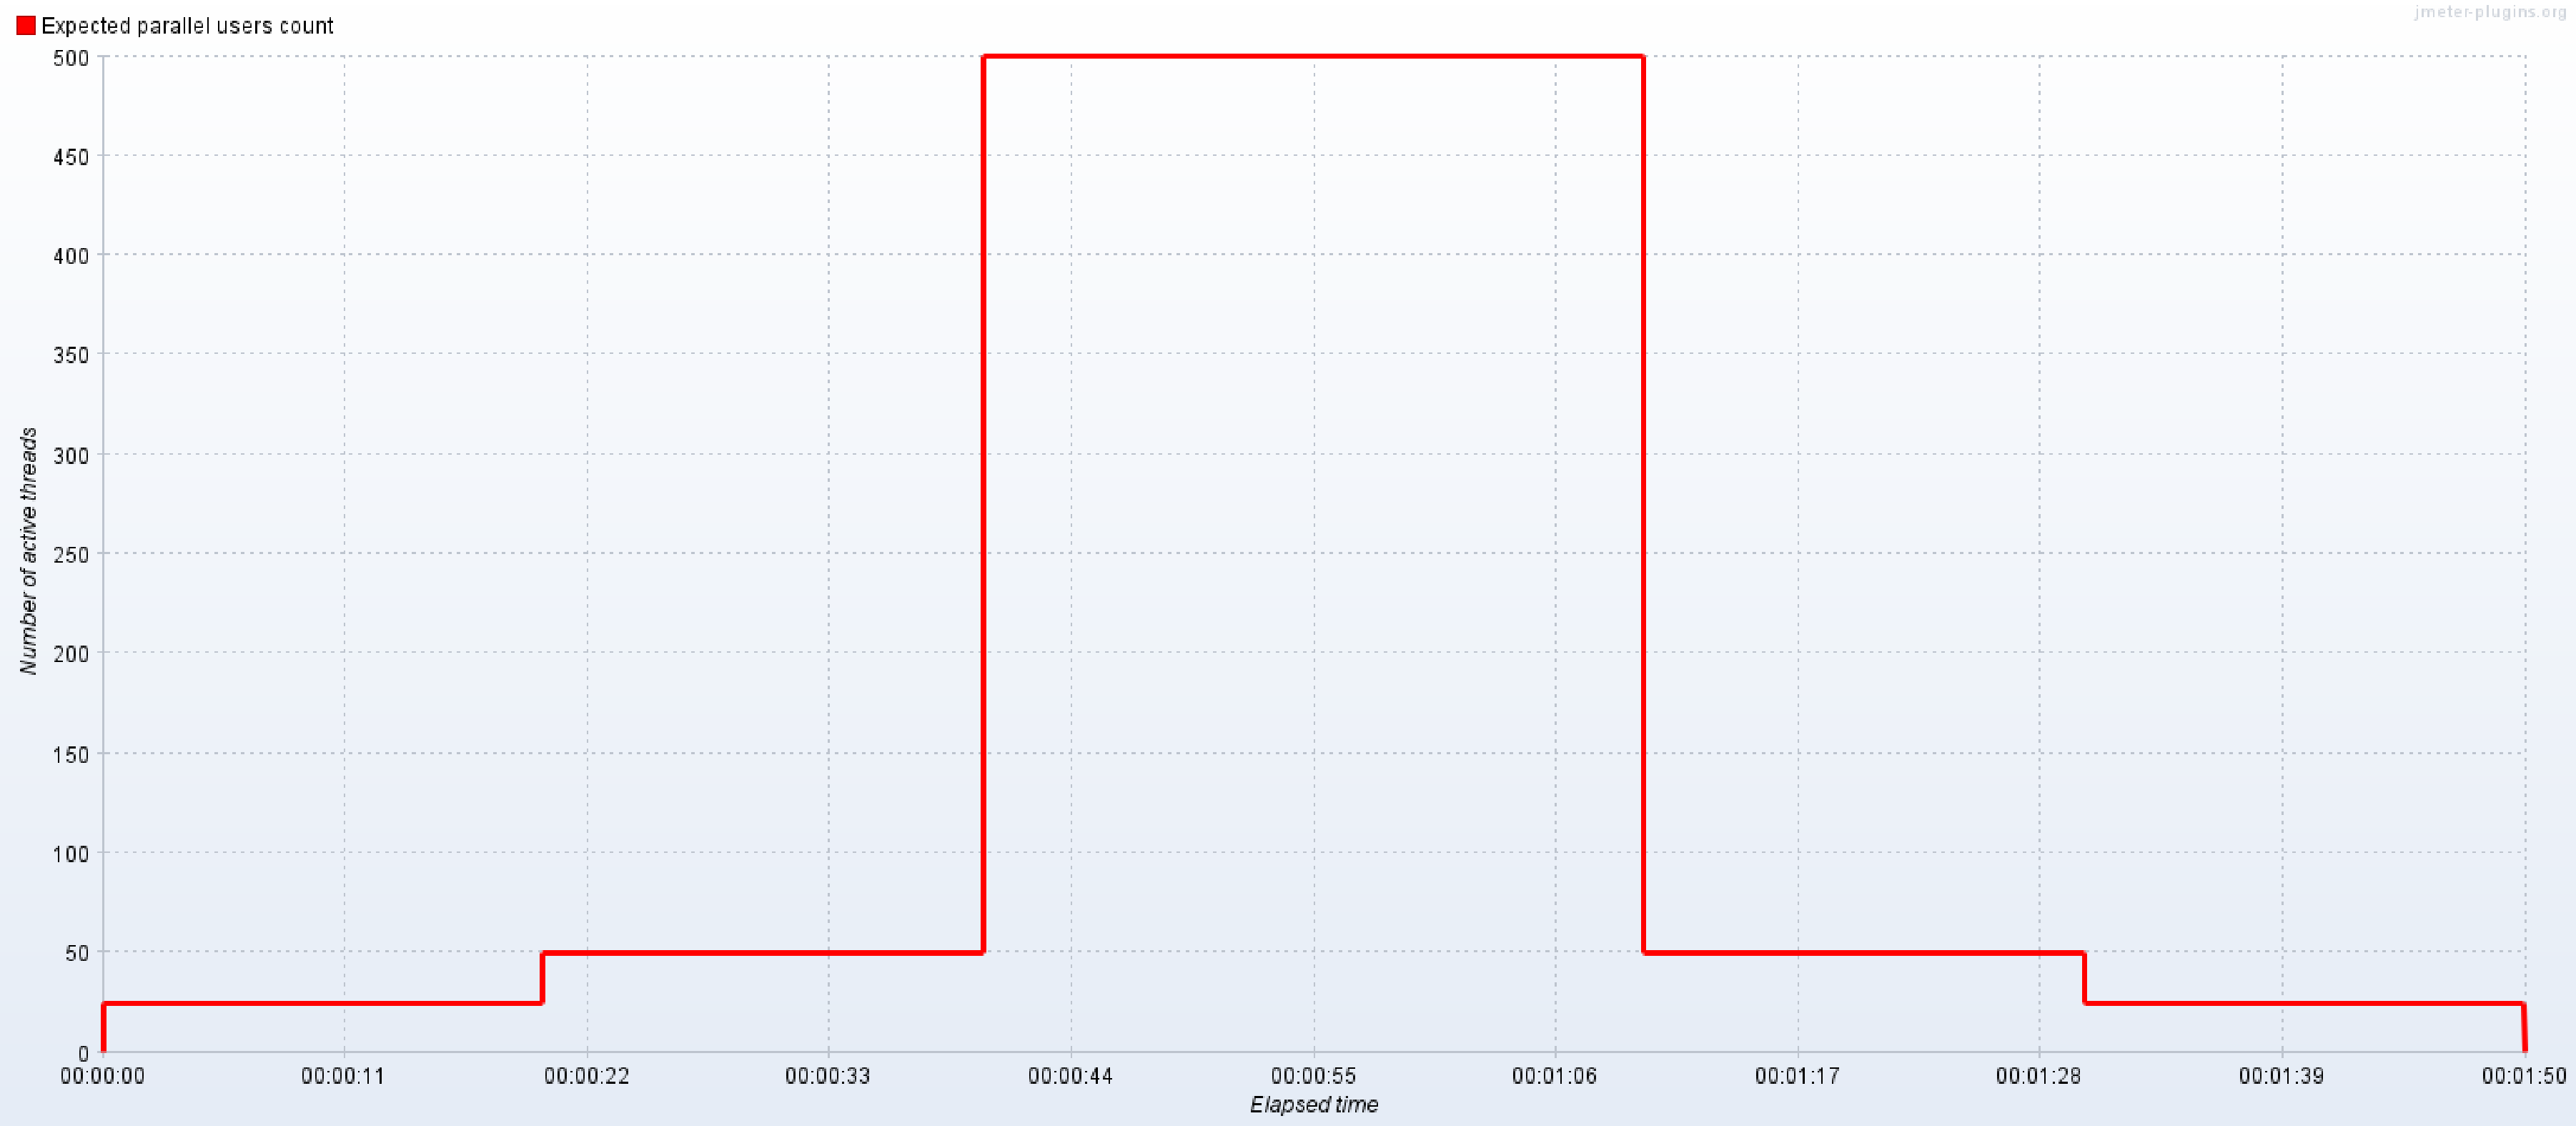
\includegraphics[width=1\linewidth]{figuras/model-spike1-v2.pdf}
%         \captionsetup{justification=centering}
%         \source{O autor.}
%         \label{fig:model-spike1}
%     \end{figure}
% \end{frame}

% \begin{frame}{Modelagem dos cenários de teste}
%     \begin{figure}[H]
%         \centering
%         \caption{Modelagem do teste de carga crescente}
%         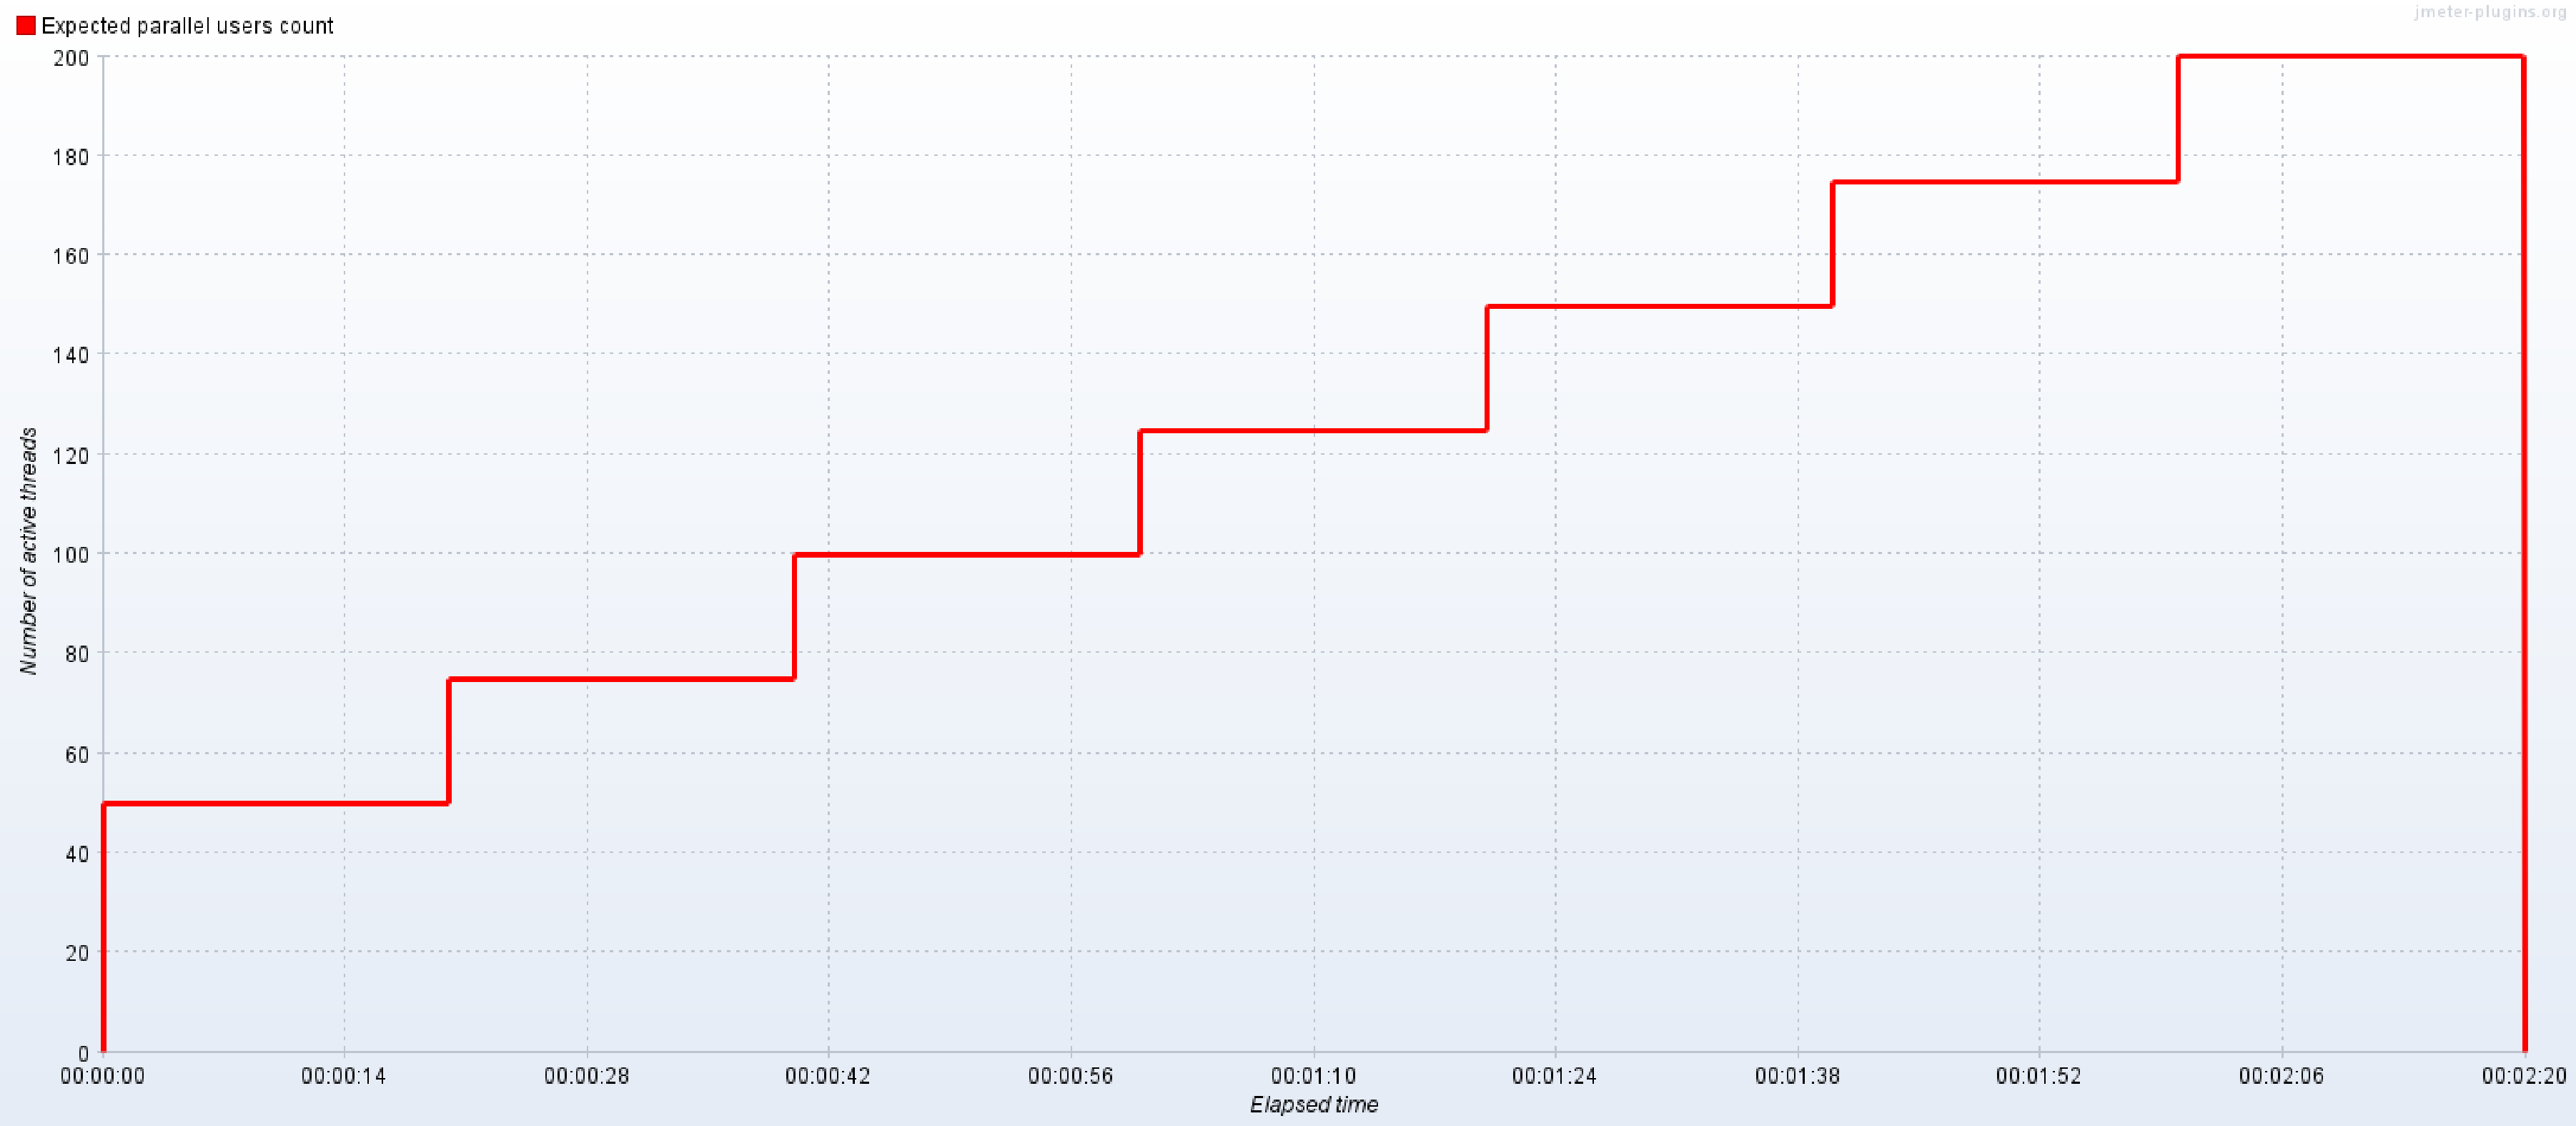
\includegraphics[width=1\linewidth]{figuras/model-crescente-v2.pdf}
%         \captionsetup{justification=centering}
%         \source{O autor.}
%         \label{fig:model-crescente}
%     \end{figure}
% \end{frame}

% \begin{frame}{Modelagem dos cenários de teste}
%     \begin{figure}[H]
%         \centering
%         \caption{Modelagem do teste de resistência}
%         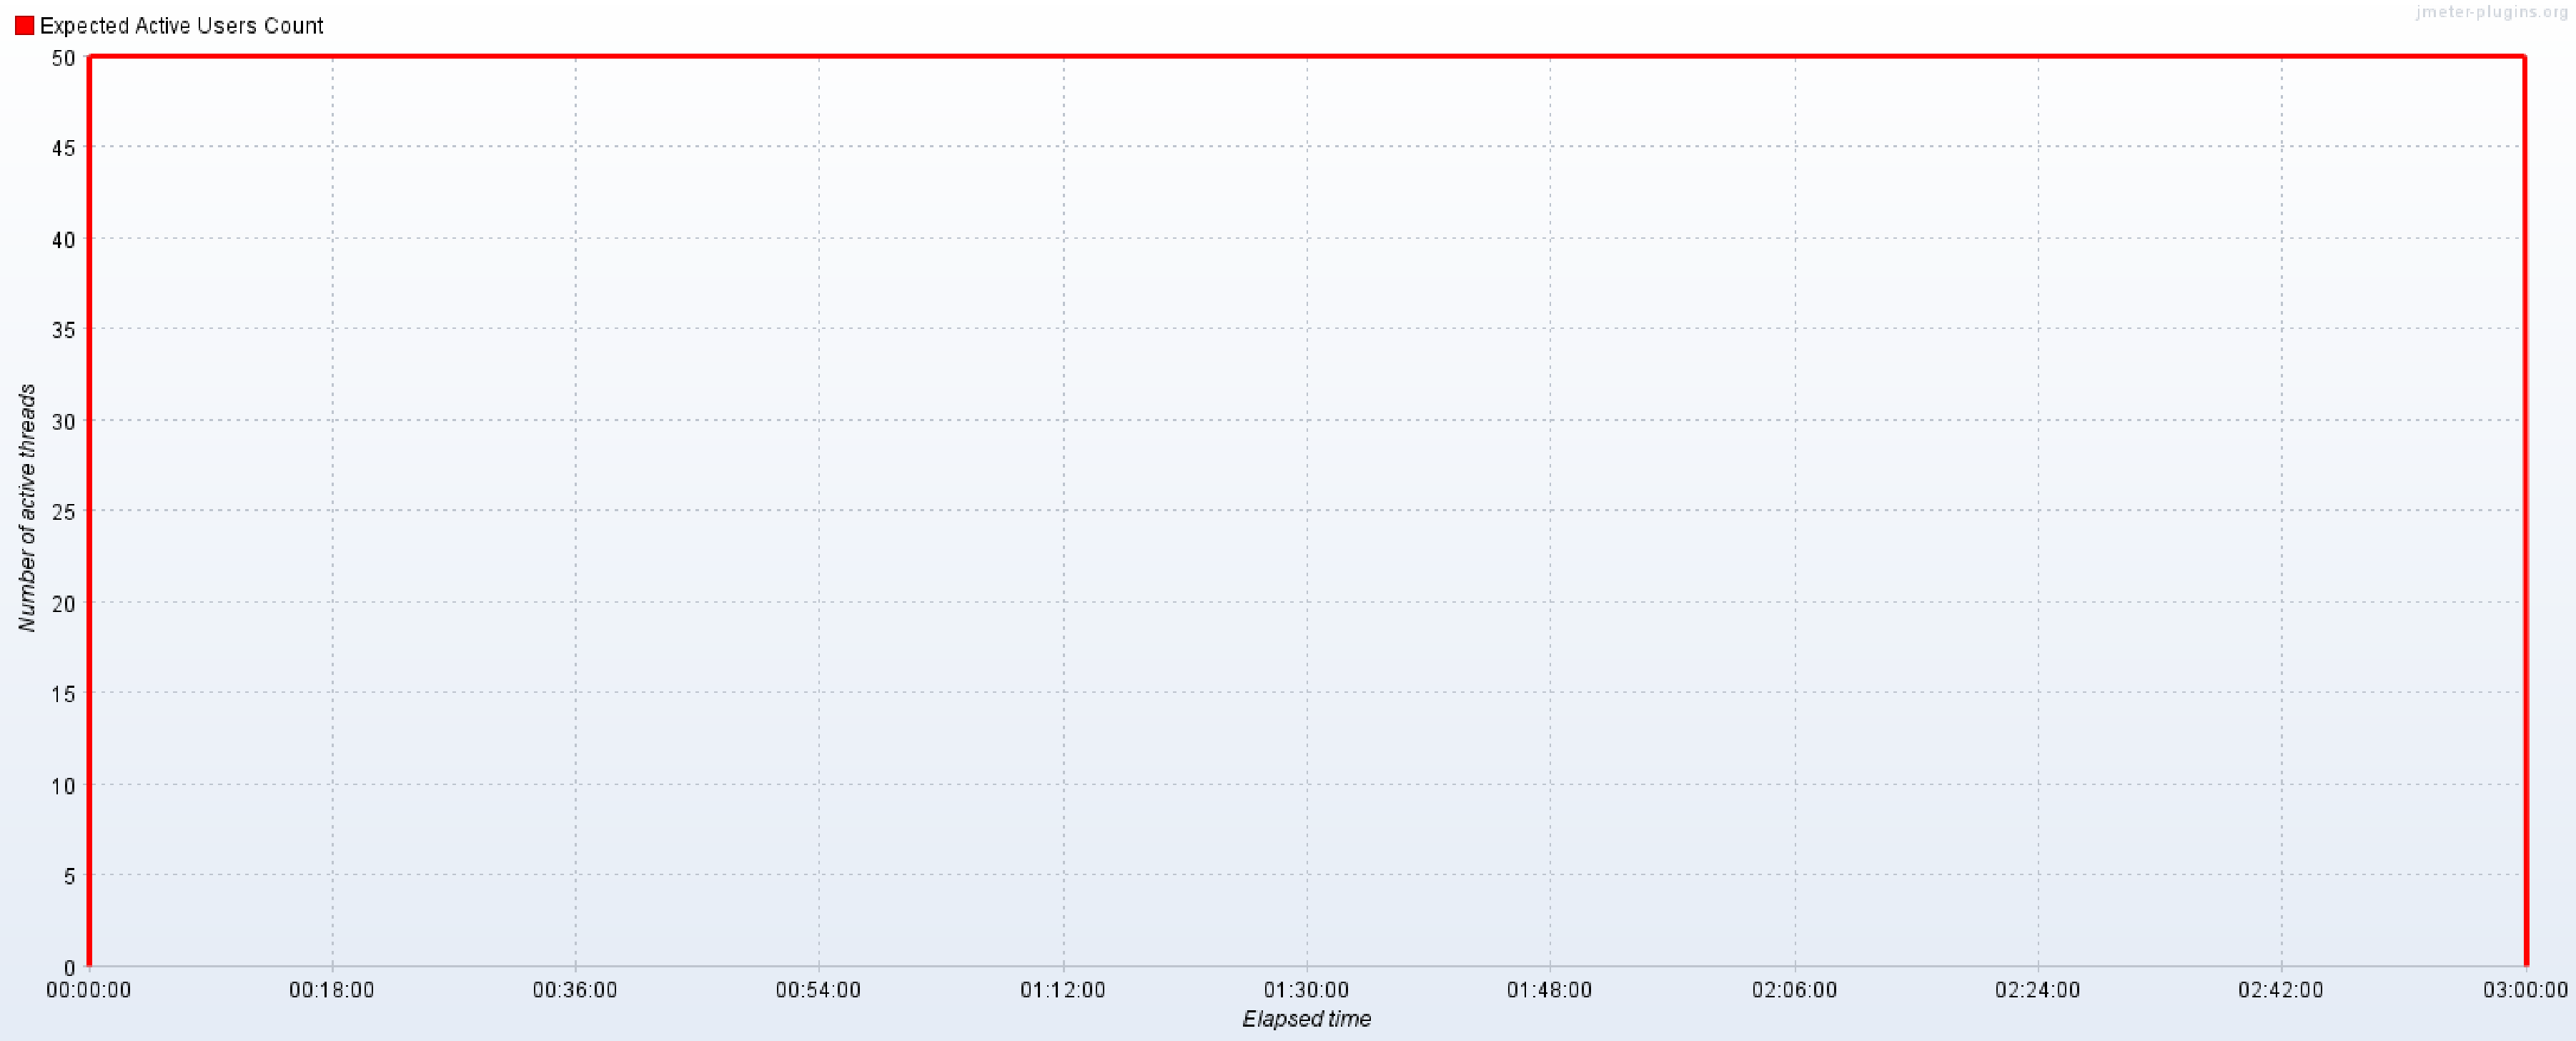
\includegraphics[width=1\linewidth]{figuras/model-endurance-v2.pdf}
%         \captionsetup{justification=centering}
%         \source{O autor.}
%         \label{fig:model-endurance}
%     \end{figure}
% \end{frame}

\begin{frame}{Execução dos testes}
    \begin{itemize}
        \item Modelagem dos testes feitos no JMeter\nocite{jmeter}\let\thefootnote\relax\footnotetext{\url{https://jmeter.apache.org/}};
            \begin{itemize}
                \item Tempo de resposta;
                \item Taxa de erros de requisição;
            \end{itemize}
        \vspace*{0.5em}
        \item Execução no Linux;
            \begin{itemize}
                \item Consumo de CPU;
                \item Consumo de RAM;
            \end{itemize}
        \vspace*{0.5em}
        \item Para a otimização do processo de testes foram utilizadas variáveis ambiente no JMeter e um \textit{script} para a execução dos testes via linha de comando;
    \end{itemize}
\end{frame}

%% ---------------------------------------------------------------------------
\section{Resultados e discussões}

\subsection{Comparação teórica}
\begin{frame}{Resultados comparação teórica}
    \begin{table}[H]
        \centering
        \begin{tabular}{|cc|c|c|c|}
        \hline
        \multicolumn{2}{|c|}{\textbf{CARACTERÍSTICAS}}                                           & \textbf{Node.js} & \textbf{DRF} & \textbf{.NET Core} \\ \hline
        \multicolumn{1}{|c|}{\multirow{3}{*}{\textbf{Sistemas operacionais}}} & \textbf{Windows} & Sim              & Sim          & Sim                   \\ \cline{2-5} 
        \multicolumn{1}{|c|}{}                                                & \textbf{Linux}   & Sim              & Sim          & Sim*                  \\ \cline{2-5} 
        \multicolumn{1}{|c|}{}                                                & \textbf{MacOS}   & Sim              & Sim          & Sim*                  \\ \hline
        \end{tabular}
        \captionsetup{justification=centering}
        \caption{Suporte das tecnologias aos principais SOs.}
        \caption*{\textit{*É importante ressaltar que apenas a estrutura do ASP.NET Core é multiplataforma, se diferenciando da estrutura .NET Framework que tem suporte apenas para o sistema operacional Windows.}}
        \label{tab:resultado-so}
    \end{table}
\end{frame}

\begin{frame}{Resultados comparação teórica}
    \begin{table}[H]
        \centering
        \begin{tabular}{|cc|c|c|c|}
        \hline
        \multicolumn{2}{|c|}{\textbf{CARACTERÍSTICAS}}                                                            & \textbf{Node.js} & \textbf{DRF} & \textbf{ASP.NET Core} \\ \hline
        \multicolumn{1}{|c|}{\multirow{5}{*}{\textbf{Banco de dados}}} & \textbf{MySQL}                           & Sim              & Sim          & Sim                   \\ \cline{2-5} 
        \multicolumn{1}{|c|}{}                                         & \textbf{PostgreSQL}                      & Sim              & Sim          & Sim                   \\ \cline{2-5} 
        \multicolumn{1}{|c|}{}                                         & \textbf{SQLite}                          & Sim              & Sim          & Sim                   \\ \cline{2-5} 
        \multicolumn{1}{|c|}{}                                         & \multicolumn{1}{l|}{\textbf{MongoDB}}    & Sim              & Não*          & Sim                   \\ \cline{2-5} 
        \multicolumn{1}{|c|}{}                                         & \multicolumn{1}{l|}{\textbf{SQL Server}} & Sim              & Sim          & Sim                   \\ \hline
        \end{tabular}
        \captionsetup{justification=centering}
        \caption{Suporte das tecnologias aos principais bancos de dados.}
        \caption*{\textit{*Bancos de dados não relacionais não são suportados nativamente pelo Django.}}
        \label{tab:resultado-bd}
    \end{table}
\end{frame}

\begin{frame}{Resultados comparação teórica}
    \begin{table}[H]
        \centering
        \begin{tabular}{|c|c|c|c|}
        \hline
        \textbf{CARACTERÍSTICAS} & \textbf{Node.js} & \textbf{DRF} & \textbf{ASP.NET Core} \\ \hline
        \textbf{ORM nativo}      & Não              & Sim          & Não                   \\ \hline
        \end{tabular}
        \captionsetup{justification=centering}
        \caption{Suporte das tecnologias ao ORM nativo}
        \label{tab:resultado-orm}
    \end{table}
\end{frame}

\begin{frame}{Resultados comparação teórica}
    \begin{table}[H]
        \centering
        \begin{tabular}{|c|c|c|c|}
        \hline
        \textbf{CARACTERÍSTICAS} & \textbf{Node.js} & \textbf{DRF} & \textbf{ASP.NET Core} \\ \hline
        \textbf{Documentação nativa}      & Não              & Não*          & Sim                   \\ \hline
        \end{tabular}
        \captionsetup{justification=centering}
        \caption{Suporte das tecnologias à documentação nativa.}
        \caption*{\textit{*A geração de documentação pelo DRF não é feita de forma automática, porém existe suporte integrado para esquemas OpenAPI.}}
        \label{tab:resultado-documentacao}
    \end{table}
\end{frame}


\begin{frame}{Resultados e discussões}
    \begin{block}{QP1: Qual é o \textit{framework} com mais funcionalidades nativas seguindo as características escolhidas para estudo?}
        De acordo com os estudos bibliográficos realizados, o DRF e o .Net apresentaram mais funcionalidades nativas. No entanto, os três \textit{framework} possuem compatibilidade para diversas funcionalidades, principalmente utilizando bibliotecas de terceiros. Portanto, os três são flexíveis para adaptação dependendo do contexto que serão utilizados.
    \end{block}
\end{frame}

\begin{frame}{Resultados - outras observações}
    \begin{itemize}
        \item Todas os \textit{framework} ofereciam suporte para a construção das APIs;
        \vspace*{0.5em}
        \item Dificuldades no desenvolvimento em .Net devido à liguagem e seu paradigma;
        \vspace*{0.5em}
        \item Flexibilidade no desenvolvimento com Node.js e DRF;
    \end{itemize}
\end{frame}


\subsection{Comparação prática}
\begin{frame}{Resultados - teste de pico}
    \begin{figure}[H]
        \centering
        \caption{Consumo médio de recursos - teste de pico}
        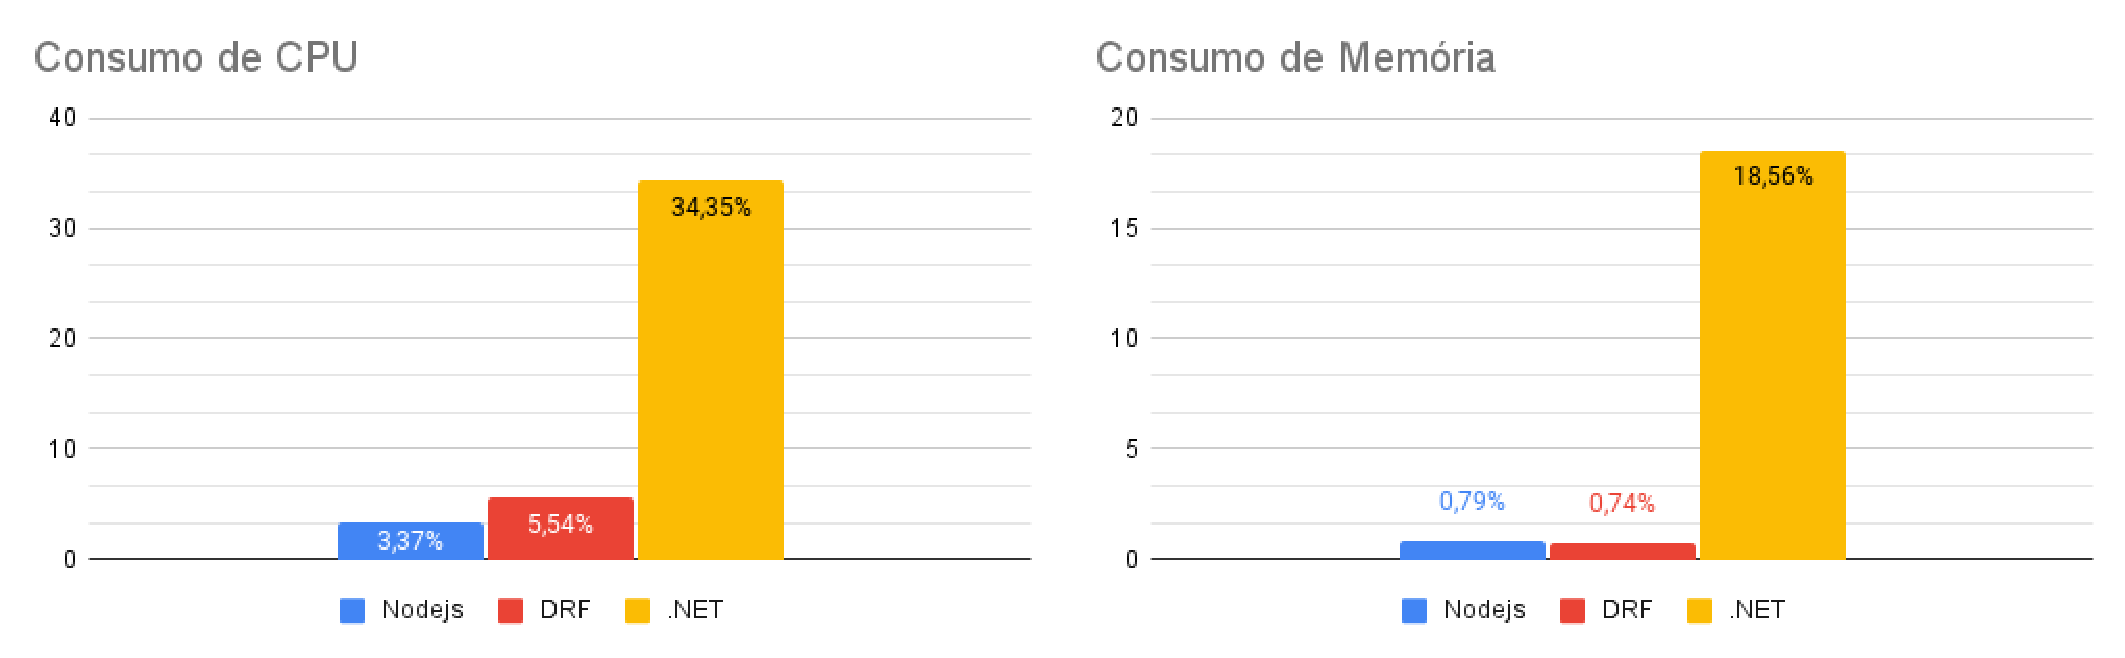
\includegraphics[width=1\linewidth]{figuras/resultados/consumo-recursos-pico.pdf}
        \captionsetup{justification=centering}
        \source{O autor.}
        \label{fig:recursos-pico}
    \end{figure}
\end{frame}

\begin{frame}{Resultados - teste de pico}
    \begin{block}{QP2: Qual é o \textit{framework} mais otimizado com relação ao consumo de recursos no cenário de teste de pico?}
        O Node.js apresentou menor consumo de CPU enquanto o DRF mostrou melhor resultado no consumo de RAM.
    \end{block}
\end{frame}

\begin{frame}{Resultados - teste de pico}
    \begin{figure}[H]
        \centering
        \caption{Tempo de resposta médio dos métodos HTTP - teste de pico}
        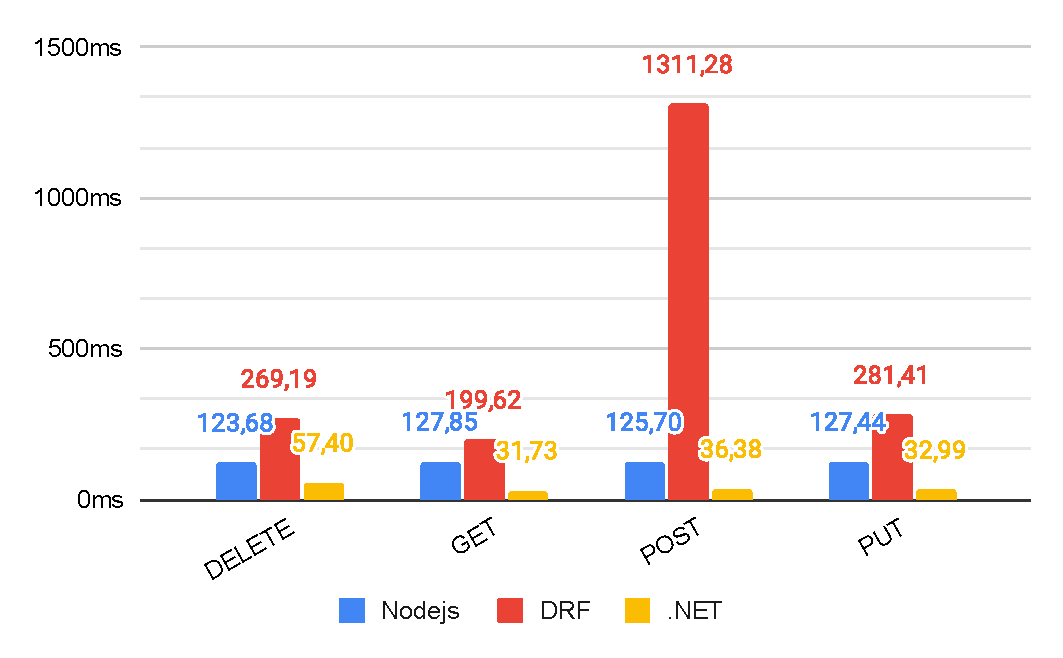
\includegraphics[width=0.9\linewidth]{figuras/resultados/spike1-tempo-metodos-totais3.pdf}
        \captionsetup{justification=centering}
        \source{O autor.}
        \label{fig:spike1-tempo-metodos-totais}
    \end{figure}
\end{frame}

\begin{frame}{Resultados - teste de pico}
    \begin{block}{QP3: Qual é o \textit{framework} mais otimizado com relação ao tempo de resposta no cenário de teste de pico?}
        O .Net apresentou os melhores resultados em tempo de resposta em todos os métodos.
    \end{block}
\end{frame}


\begin{frame}{Resultados - teste de carga crescente}
    \begin{figure}[H]
        \centering
        \caption{Consumo médio recursos - teste de carga crescente}
        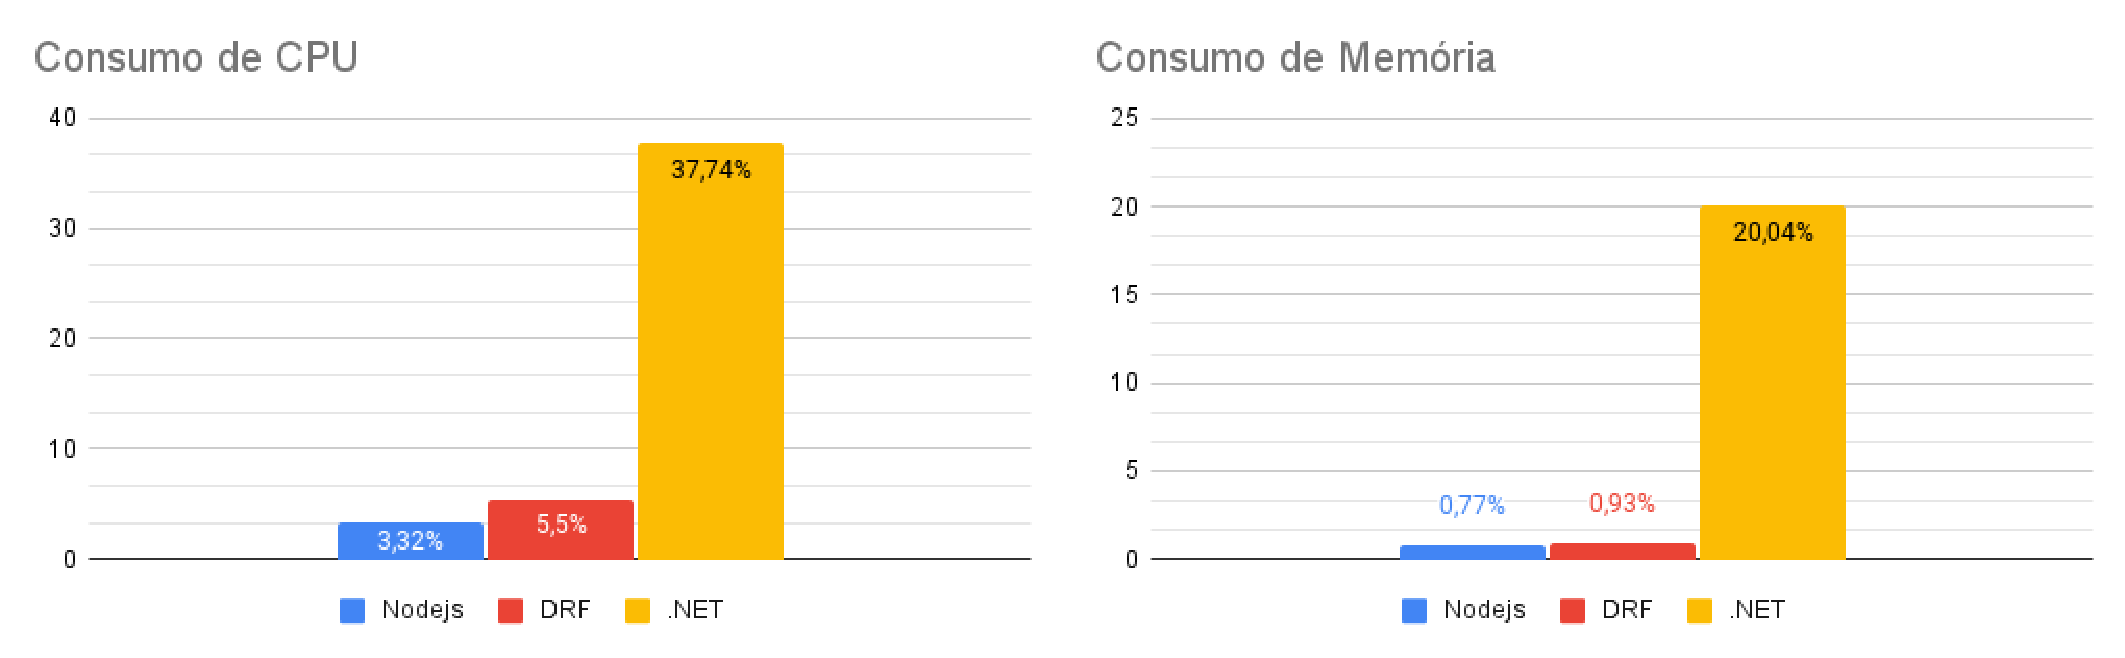
\includegraphics[width=1\linewidth]{figuras/resultados/consumo-recursos-crescente.pdf}
        \captionsetup{justification=centering}
        \source{O autor.}
        \label{fig:recursos-crescente}
    \end{figure}
\end{frame}

\begin{frame}{Resultados - teste de carga crescente}
    \begin{block}{QP4: Qual é o \textit{framework} mais otimizado com relação ao consumo de recursos no cenário de teste de carga crescente?}
        O Node.js apresentou os melhores resultados, tanto para consumo de CPU quando RAM.
    \end{block}
\end{frame}

\begin{frame}{Resultados - teste de carga crescente}
    \begin{figure}[H]
        \centering
        \caption{Tempo de resposta médio dos métodos HTTP - teste de carga crescente}
        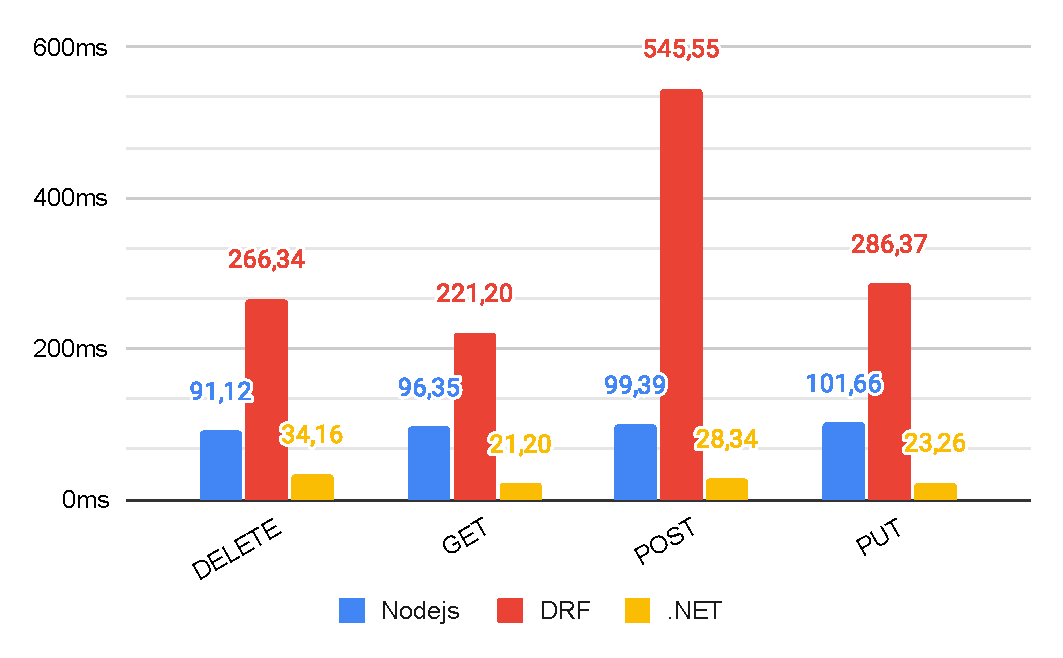
\includegraphics[width=0.9\linewidth]{figuras/resultados/crescente-tempo-metodos-totais3.pdf}
        \captionsetup{justification=centering}
        \source{O autor.}
        \label{fig:crescente-tempo-metodos-totais}
    \end{figure}
\end{frame}

\begin{frame}{Resultados - teste de carga crescente}
    \begin{block}{QP5: Qual é o \textit{framework} mais otimizado com relação ao tempo de resposta no cenário de teste de carga crescente?}
        O .Net apresentou os melhores resultados em tempo de resposta em todos os métodos no cenário de carga crescente.
    \end{block}
\end{frame}


\begin{frame}{Resultados - teste de resistência}
    \begin{figure}[H]
        \centering
        \caption{Consumo médio de recursos - teste de resistência}
        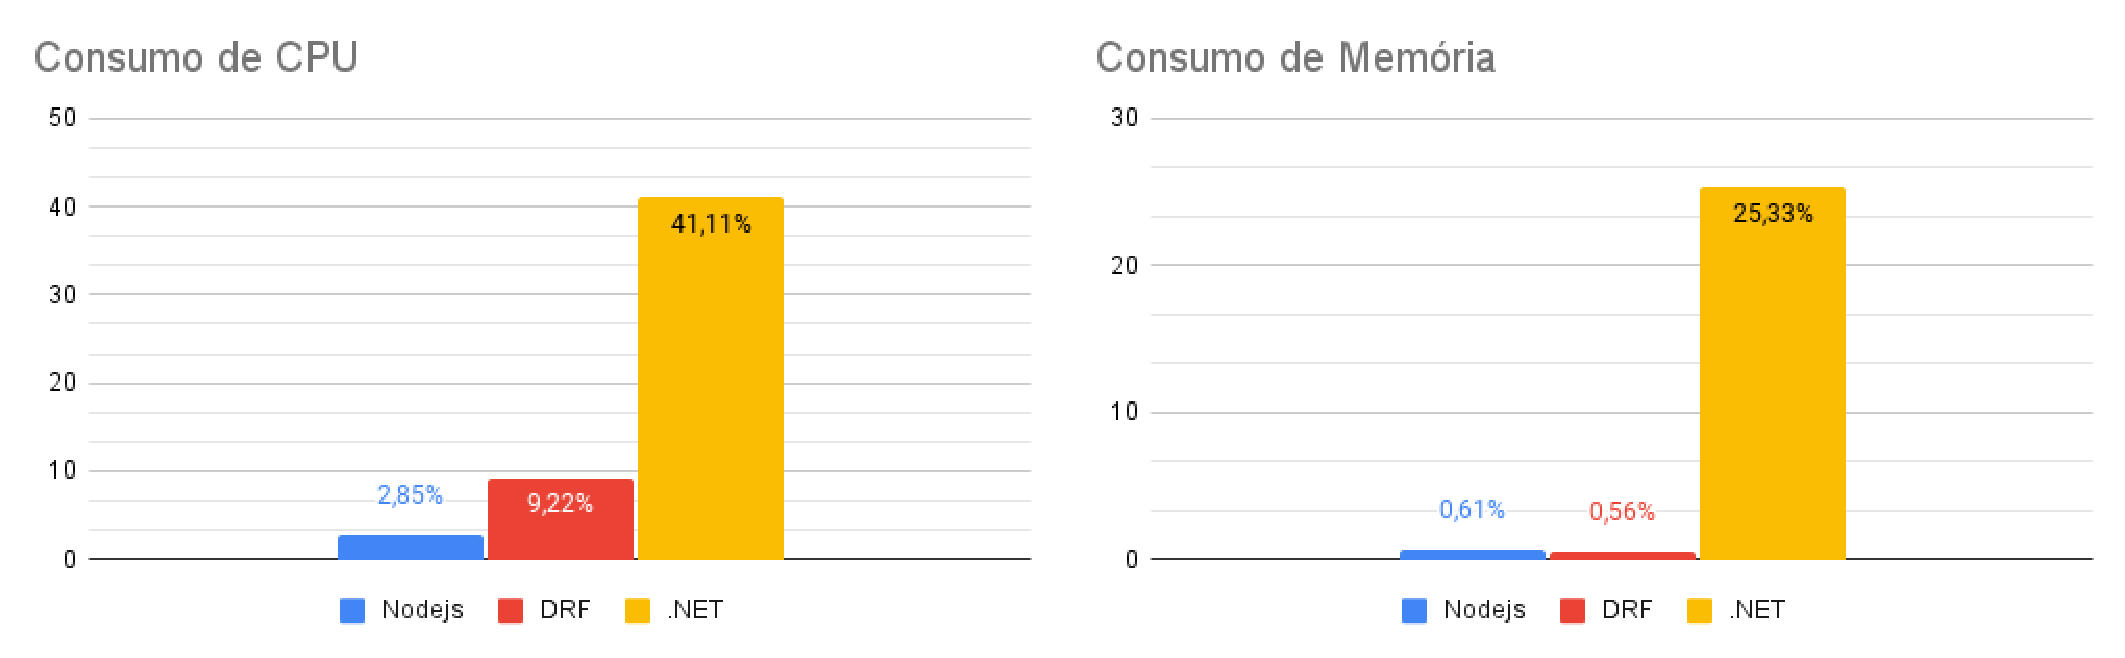
\includegraphics[width=1\linewidth]{figuras/resultados/consumo-recursos-resistencia.pdf}
        \captionsetup{justification=centering}
        \source{O autor.}
        \label{fig:recursos-resistencia}
    \end{figure}
\end{frame}

\begin{frame}{Resultados - teste de resistência}
    \begin{block}{QP6: Qual é o \textit{framework} mais otimizado com relação ao consumo de recursos no cenário de teste de resistência?}
        Assim como na QP2, o Node.js apresentou menor consumo de CPU enquanto o DRF mostrou melhor resultado no consumo de RAM.
    \end{block}
\end{frame}

\begin{frame}{Resultados - teste de resistência}
    \begin{figure}[H]
        \centering
        \caption{Tempo de resposta médio dos métodos HTTP - teste de resistência}
        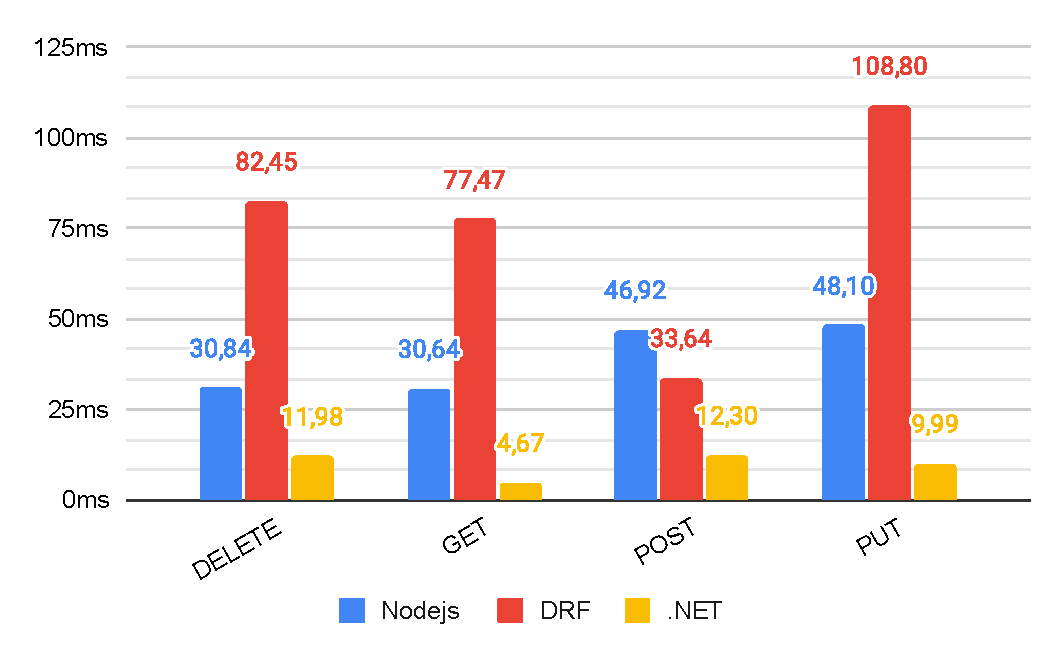
\includegraphics[width=0.9\linewidth]{figuras/resultados/endurance-tempo-metodos-totais3.pdf}
        \captionsetup{justification=centering}
        \source{O autor.}
        \label{fig:endurance-tempo-metodos-totais}
    \end{figure}
\end{frame}

\begin{frame}{Resultados - teste de carga crescente}
    \begin{block}{QP7: Qual é o \textit{framework} mais otimizado com relação ao tempo de resposta no cenário de teste de resistência?}
        O .Net apresentou os melhores resultados em tempo de resposta em todos os métodos no cenário de resistência.
    \end{block}
\end{frame}

% \subsection{Outras observações - resultados práticos}
\begin{frame}{Resultados - outras observações}
    \textbf{Taxa de erros de requisições}
    \begin{itemize}
        \item Foi observado, durante os testes práticos, que nenhum dos \textit{framework} demonstrou falhas nas requisições. Em todos os cenários avaliados, a taxa de erros de requisição foi igual a 0. Com estes resultados conclui-se que, para os cenários modelados, os \textit{framework} possuem bom rendimento.
    \end{itemize}
    
\end{frame}

\begin{frame}{Resultados - outras observações}
    \begin{figure}[H]
        \centering
        \caption{Inicialização do .Net no teste de carga crescente}
        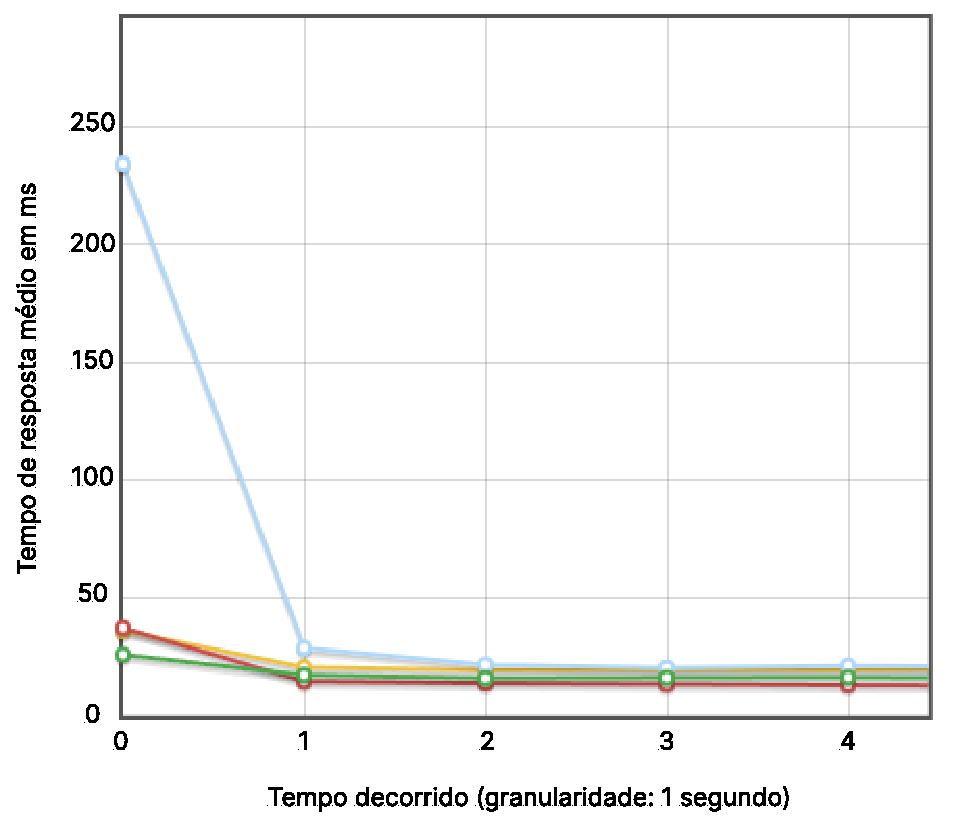
\includegraphics[width=0.65\linewidth]{figuras/resultados/start-dotnet-crescente-ex2.pdf}
        \captionsetup{justification=centering}
        \source{O autor.}
        \label{fig:endurance-tempo-metodos-totais}
    \end{figure}
\end{frame}

%% ---------------------------------------------------------------------------
\section{Contribuições}
\begin{frame}{Contribuições}
    \textbf{O presente estudo foi submetido em formato de artigo no SBSI 2024}
    \begin{itemize}
        \item XX Simpósio Brasileiro de Sistemas de Informação;
    \end{itemize}
    \begin{figure}[H]
        \centering
        \caption{SBSI 2024}
        
\includegraphics[width=0.6\linewidth]{figuras/sbsi2024.png}
        \captionsetup{justification=centering}
        \source{\href{https://sbsi2024.ufjf.br/}{Simpósio Brasileiro de Sistemas de Informação}}
        \label{fig:model-endurance}
    \end{figure}
\end{frame}
 

%% ---------------------------------------------------------------------------
\section{Conclusões e trabalhos futuros}

\begin{frame}{Conclusões e trabalhos futuros}
    \textbf{Conclusões comparação teórica}
    \begin{itemize}
        \item Cada \textit{framework} apresenta diferentes funcionalidades nativas;
        \vspace*{0.5em}
        \item Apesar das diferenças, todos podem ser configurados para adequar às necessidades de um projeto.
    \end{itemize}
\end{frame}

\begin{frame}{Conclusões e trabalhos futuros}
    \textbf{Conclusões comparação prática}
    \begin{itemize}
        \item Nenhum \textit{framework} apresentou erros de requisição;
        \vspace*{0.5em}
        \item Node.js e Django REST Framework com melhores resultados em consumo de recursos;
        \vspace*{0.5em}
        \item .Net Core apresentou melhores resultados com relação ao tempo de resposta.
    \end{itemize}
\end{frame}

\begin{frame}{Conclusões e trabalhos futuros}
    \textbf{Trabalhos futuros}
    \begin{itemize}
        \item Utilização de outros bancos de dados;
        \vspace*{0.5em}
        \item Reaplicação dos testes em outros cenários;
        \vspace*{0.5em}
        \item Reaplicação dos testes simulando outras funcionalidades.
    \end{itemize}
\end{frame}

%% ---------------------------------------------------------------------------
% Reference frames
\begin{frame}[allowframebreaks]
    \frametitle{Referências}
    \printbibliography
\end{frame}

%% ---------------------------------------------------------------------------
% Final frame
\begin{frame}{}
    \centering
    \huge{\textbf{\example{Obrigado(a) pela Atenção!}}}
    
    \vspace{1cm}
    
    \Large{\textbf{Contato:}}
    \newline
    \vspace*{0.5cm}
    \large{\email{klayver@alu.ufc.br}}
\end{frame}

%% ---------------------------------------------------------------------------

\begin{comment}

\section{Modelos}
\begin{frame}{Modelos}
    % itemize
    Este é um template que pode ser utilizado para:
    \begin{itemize}
        \item Apresentação de Trabalhos Acadêmicos
        \item Apresentação de Disciplinas
        \item Apresentações de Teses e Dissertações
    \end{itemize}

    \vspace{0.4cm} % vertical space
    
    % enumeration
    Para utilizar este template corretamente é importante que:
    \begin{enumerate}
        \item Tenha conhecimento mínimo sobre LaTeX
        \item Ler os comentários no template (explicações)
        \item Ler o README.md (documentação)
    \end{enumerate}

    \vspace{0.2cm}

    \example{Este é um texto de exemplo!} \emph{Texto de Ênfase!}
\end{frame}

%% ---------------------------------------------------------------------------
\subsection{Subseção I}
\begin{frame}{Criando Blocos}
    % Blocks styles
    \begin{block}{Bloco Padrão}
        Texto do corpo do bloco.
    \end{block}

    \begin{alertblock}{Bloco de Alerta}
        Texto do corpo do bloco.
    \end{alertblock}

    \begin{exampleblock}{Bloco de Exemplo}
        Texto do corpo do bloco.
    \end{exampleblock}   
\end{frame}

%% ---------------------------------------------------------------------------
\subsection{Subseção II}
\begin{frame}{Criando Caixas}
    \successbox{testando o success box}

    \pause

    \alertbox{testando o alert box}

    \pause

    \simplebox{testando o simple box}
\end{frame}

%% ---------------------------------------------------------------------------
\subsection{Subseção III}
\begin{frame}{Criando Algoritmos (Pseudocódigo)}
    \begin{algorithm}[H]
        \SetAlgoLined
        \LinesNumbered
        \SetKwInOut{Input}{input}
        \SetKwInOut{Output}{output}
        \Input{x: float, y: float}
        \Output{r: float}
        \While{True}{
          r = x + y\;
          \eIf{r >= 30}{
           ``O valor de $r$ é maior ou iqual a 10.''\;
           break\;
           }{
           ``O valor de $r$ = '', r\;
          }
         } 
         \caption{Algorithm Example}
    \end{algorithm}
\end{frame}

%% ---------------------------------------------------------------------------

\begin{frame}{Inserindo Algoritmos}
    \lstset{language=Python}
    \lstinputlisting[language=Python]{code/main.py}
\end{frame}

%% ---------------------------------------------------------------------------
\begin{frame}{Inserindo Algoritmos}
    \lstinputlisting[language=C]{code/source.c}
\end{frame}

%% ---------------------------------------------------------------------------
\begin{frame}{Inserindo Algoritmos}
    \lstinputlisting[language=Java]{code/helloworld.java}
\end{frame}

%% ---------------------------------------------------------------------------
\begin{frame}{Inserindo Algoritmos}
    \lstinputlisting[language=HTML]{code/index.html}
\end{frame}

%% ---------------------------------------------------------------------------
% This frame show an example to insert multicolumns
\section{Multicolunas}
\begin{frame}{Seção II - Multicolunas}
    \begin{columns}{}
        \begin{column}{0.5\textwidth}
            \justify
            É possível colocar mais de uma coluna utilizando os comandos de $\backslash$begin\{column\}\{\} e $\backslash$end\{column\}
        \end{column}
        \begin{column}{0.5\textwidth}
            \justify
            Porém, o espaçamento deve ser proporcional entre as colunas para que estas colunas não entrem em coflito. O espaçamento é dado pelo segundo argumento do $\backslash$begin.
        \end{column}
    \end{columns}    
\end{frame}

%% ---------------------------------------------------------------------------
% This frame show an example to insert figures
\section{Imagens}
\begin{frame}{Seção III - Figures}
    \begin{figure}
        \centering
        \caption{Emblema da UFC.}
        
\includegraphics[scale=0.3]{libs/emblemufc.pdf}
        \source{Obtido pelo site oficial da UFC \cite{siteufc} \cite{einstein}}
        \label{fig:ufc_emblem}
    \end{figure}
\end{frame}
\end{comment}


\end{document}
